\noindent
\begin{minipage}[t]{0.28\textwidth}
    \vspace{0pt}
    \vspace{6pt}
    % Hộp lịch sử Cauchy và Giới hạn ở lề trái
    \begin{tcolorbox}[
        colback=white,
        colframe=stewartgreen,
        arc=0mm,
        boxrule=1pt,
        left=6pt,
        right=6pt,
        top=7pt,
        bottom=7pt,
        boxsep=0pt
    ]
    {\fontsize{10pt}{12.5pt}\selectfont\textbf{\textsf{\color{stewartgreen}Cauchy và Giới hạn}}}\par\vspace{5pt}
    {\fontsize{7.9pt}{10.8pt}\selectfont
    Sau phát minh về phép tính vi tích phân vào thế kỷ 17, đã diễn ra một giai đoạn phát triển tự do của bộ môn này trong thế kỷ 18. Các nhà toán học như anh em nhà Bernoulli và Euler rất háo hức khai thác sức mạnh của giải tích và mạnh dạn khám phá những hệ quả từ lý thuyết toán học mới mẻ và kỳ diệu này mà không quá bận tâm về việc liệu các chứng minh của họ có hoàn toàn chính xác hay không.\par\vspace{5pt}
    Trái lại, thế kỷ 19 là Thời đại của sự Chặt chẽ trong toán học. Đã xuất hiện một phong trào quay trở lại với các nền tảng của bộ môn—nhằm đưa ra những định nghĩa cẩn trọng và các chứng minh chặt chẽ. Đi đầu trong phong trào này là nhà toán học người Pháp Augustin-Louis Cauchy (1789--1857), người khởi đầu là một kỹ sư quân sự trước khi trở thành giáo sư toán học tại Paris. Cauchy đã tiếp thu ý tưởng của Newton về giới hạn, vốn được duy trì trong thế kỷ 18 bởi nhà toán học người Pháp Jean d'Alembert, và làm cho nó trở nên chính xác hơn. Định nghĩa của ông về giới hạn như sau: ``Khi các giá trị liên tiếp gán cho một biến số tiến gần vô hạn đến một giá trị cố định sao cho khoảng cách sai khác cuối cùng nhỏ tùy ý theo mong muốn, thì giá trị cố định này được gọi là \textit{giới hạn} của tất cả các giá trị kia.'' Nhưng khi Cauchy sử dụng định nghĩa này trong các ví dụ và chứng minh, ông thường sử dụng các bất đẳng thức delta-epsilon tương tự như những bất đẳng thức trong mục này. Một chứng minh điển hình của Cauchy bắt đầu bằng: ``Ký hiệu $\delta$ và $\varepsilon$ là hai số rất nhỏ; \dots'' Ông dùng $\varepsilon$ vì sự tương ứng giữa chữ cái epsilon và từ tiếng Pháp \textit{erreur} (sai số), và dùng $\delta$ vì delta tương ứng với từ \textit{différence} (hiệu số). Sau này, nhà toán học người Đức Karl Weierstrass (1815--1897) đã phát biểu định nghĩa giới hạn hoàn toàn trùng khớp với Định nghĩa 2 của chúng ta.\par}
    \end{tcolorbox}
\end{minipage}%
\hfill
\begin{minipage}[t]{0.68\textwidth}
    \vspace{0pt}
    Nhưng $|(4x - 5) - 7| = |4x - 12| = |4(x - 3)| = 4|x - 3|$. Do đó ta muốn tìm $\delta$ sao cho
    \begin{equation*}
    \begin{array}{rll}
    & \text{nếu}\quad 0 < |x - 3| < \delta \quad\text{thì} & 4|x - 3| < \varepsilon \\[4pt]
    \text{tức là,}\quad & \text{nếu}\quad 0 < |x - 3| < \delta \quad\text{thì} & |x - 3| < \dfrac{\varepsilon}{4}
    \end{array}
    \end{equation*}
    Điều này gợi ý rằng chúng ta nên chọn $\delta = \varepsilon/4$.

    \vspace{0.3em}
    \textbf{2.}\ \textit{Chứng minh (chỉ ra rằng giá trị $\delta$ này thỏa mãn).}\ Cho trước $\varepsilon > 0$, chọn $\delta = \varepsilon/4$. Nếu $0 < |x - 3| < \delta$, thì
    \[
    |(4x - 5) - 7| = |4x - 12| = 4|x - 3| < 4\delta = 4\left(\frac{\varepsilon}{4}\right) = \varepsilon
    \]
    Do đó
    \[
    \text{nếu}\qquad 0 < |x - 3| < \delta \qquad\text{thì}\qquad |(4x - 5) - 7| < \varepsilon
    \]
    Vì vậy, theo định nghĩa của giới hạn,
    \[
    \lim_{x \to 3} (4x - 5) = 7
    \]
    Ví dụ này được minh họa bởi Hình 9.

    \vspace{0.4em}
    \noindent
    \begin{minipage}[b]{0.18\textwidth}
        \textbf{\textsf{HÌNH 9}}
        \vspace{4pt}
    \end{minipage}%
    \hfill
    \begin{minipage}[b]{0.64\textwidth}
        \centering
        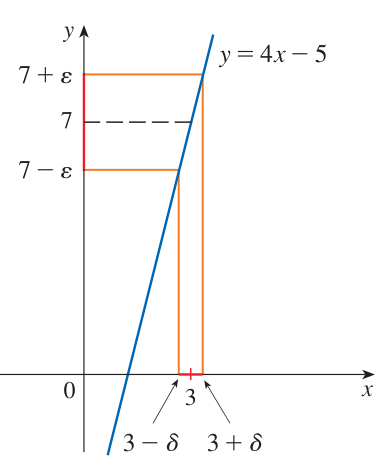
\includegraphics[width=0.72\linewidth]{images/p0144_fig1.png}
    \end{minipage}%
    \hfill
    \begin{minipage}[b]{0.14\textwidth}
        \raggedleft
        {\color{stewartcyan}\rule{1.15ex}{1.15ex}}
        \vspace{4pt}
    \end{minipage}
    \vspace{0.6em}

    Lưu ý rằng trong lời giải của Ví dụ 2 có hai giai đoạn—dự đoán và chứng minh. Chúng ta đã thực hiện một phân tích sơ bộ cho phép đoán một giá trị cho $\delta$. Nhưng sau đó ở giai đoạn thứ hai, chúng ta phải quay lại và chứng minh theo cách cẩn trọng, hợp logic rằng ta đã dự đoán đúng. Quy trình này là điển hình cho phần lớn toán học. Đôi khi cần phải đưa ra một dự đoán thông minh về lời giải cho một bài toán trước rồi sau đó mới chứng minh rằng dự đoán đó là đúng.

    \vspace{1.2em}
    \noindent{\color{stewartcyan}\textbf{\textsf{VÍ DỤ 3}}}\hspace{1.2em}Chứng minh rằng $\lim_{x \to 3} x^2 = 9$.

    \vspace{0.4em}
    \noindent{\color{stewartcyan}\textbf{\textsf{LỜI GIẢI}}}

    \vspace{0.3em}
    \textbf{1.}\ \textit{Dự đoán một giá trị cho $\delta$.}\ Cho trước $\varepsilon > 0$. Ta phải tìm một số $\delta > 0$ sao cho
    \[
    \text{nếu}\qquad 0 < |x - 3| < \delta \qquad\text{thì}\qquad |x^2 - 9| < \varepsilon
    \]
    Để liên hệ $|x^2 - 9|$ với $|x - 3|$, ta viết $|x^2 - 9| = |(x + 3)(x - 3)|$. Khi đó ta muốn
    \[
    \text{nếu}\qquad 0 < |x - 3| < \delta \qquad\text{thì}\qquad |x + 3||x - 3| < \varepsilon
    \]
\end{minipage}
